\section{Grid meta data structures}
\label{section:grid}

Various speedup techniques such as linked-cell lists \cite{xxx} and Verlet lists
\cite{xxxx} reduce the quadratic complexity in DEM codes.
Notably inspiration in this context stems from the molecular dynamics community
\cite{mattutis:24,wolfgang}. 
In the present paper, we propose to rely on a generalised tree-based linked-cell
technique that allows us to efficiently treat particles of a vast range of diameters.
Three observations support this design decision:
First, particles colliding with other particles are close to these particles.
It thus is sufficient to scan a certain environment around each particle for
potential collision partners.
We do not have to run through all particles per particle.
We thus split up the domain into control volumes.
They are cubic as this simplifies the implementation compared to control volumes
of more flexible shapes.
Second, we may choose these control volumes to be larger than the biggest
particle diameter. 
For a particle held in a particular control volume (cell), it is thus sufficient
to check the $3^d-1$ neighbouring cells whether they host other particles that
might collide. 
$d$ is the spatial dimension.
Third, the previous decision is problematic if the particles are of extremely
different size. 
The cell size is determined by the largest particle diameter. 
If we use a uniform cell size, many uneccessary collision checks are performed
for small particles.
If we use an adaptive grid, it is tricky to design the grid such that only
direct neighbouring cells have to be studied.
We thus, third, observe that a cascade of grids might be useful: If we have
several grids embedded into each other, we can store each particle in the grid
suiting its diameter.
Particles of one grid then have to be checked agains particles in their
neighbouring cell as well as neighbouring cells on coarser grid resolution
levels.
There is no need to check a particle of one grid resolution with particles of a
finer grid resolution---if a particle $A$ collides with a particle $B$, particle
$B$ also collides with particle $A$ and such relations thus are already
detected.


Alternative approaches select the mesh size to accomodate the minimal particle
diameter \cite{mattutis}.
In this case, larger particles overlap multiple cells.
Such an approach requires more sophisticated bookkeeping of particle-cell
relations. 
The idea is not followed up here.
Instead, we prioritise algorithm simplicity---a property that is notably enabled
through trees decomposing the computational domain.


A spacetree is a space-partitioning data structure constructed recursively.
The computational domain is embedded into a unit cube.
We cut the unit cube into three equidistant pieces along each coordinate axis. 
This yields 27 new cubes. 
They are called children of the bounding box cube which is the root.
For each of the children, we continue recursively to evaluate the split
decision. 
The decision to cut into three parts results from the fact that we rely on a
code base based upon three-partitioning \cite{Software:Peano}.
Bipartitioning, i.e.~the classic octree, works as well.


The construction scheme yields a cascade of ragged regular Cartesian grids that
are embedded into each other.
Each cell besides the root has a unique parent cell.
While we could make the cells hold particles, we propose to use a
multiscale, vertex-based scheme spanning a dual meta grid
\cite{Weinzierl:16:PIC}.
A vertex is unique through its spatial position plus its level. 
The level is the number of refinement steps required at least to create one of
its adjacent cells.
Each vertex holds a list of particles.
A particles is always stored on the finest grid level where the cells' edge
length is still bigger than its diameter.
A particle is always associated to the vertex next to its geometric centre,
i.e.~any vertex has a list of all particles close to it on the same level.
Links from the vertices to the particles are realised as pointers. 
If a particle moves, we have to update the links, but we do not move
geometric data in memory.


{\bf Grid traversal.}
With a grid at hand, we may map the algorithmic steps from Algorithm
\ref{algorithm:dem-blueprint} onto a grid traversal.
For the traversal, we rely on a combination of a depth-first order with
space-filling curve \cite{Weinzierl:2009:Diss,Weinzierl:11:Peano}.
From a DEM point of view, the exact traversal realisation however is not that
relevant as long as the traversal is a real tree traversal, i.e.~runs through
all levels of the underlying spacetree.

\begin{figure}
  \begin{center}
    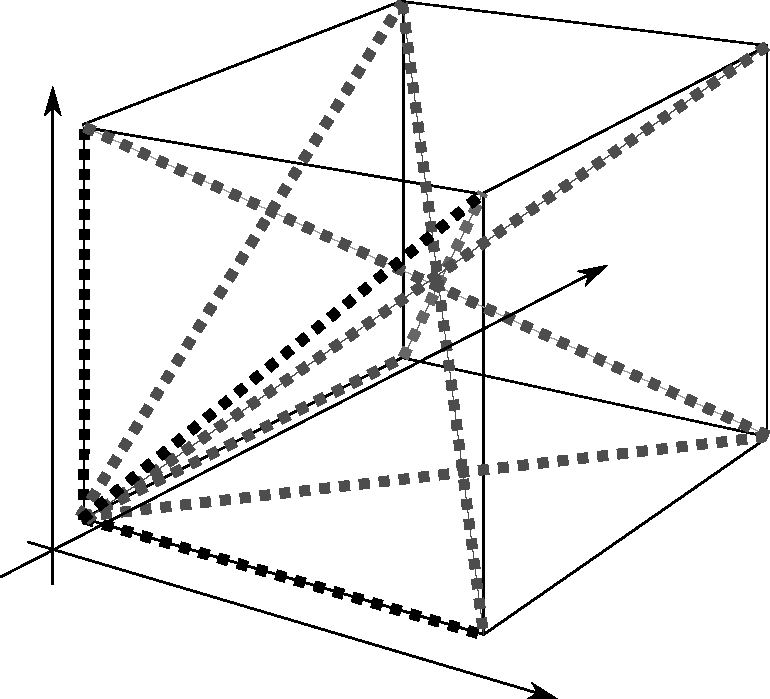
\includegraphics[width=0.25\textwidth]{sketches/collision-cube.pdf}
    \hspace{0.2cm}
    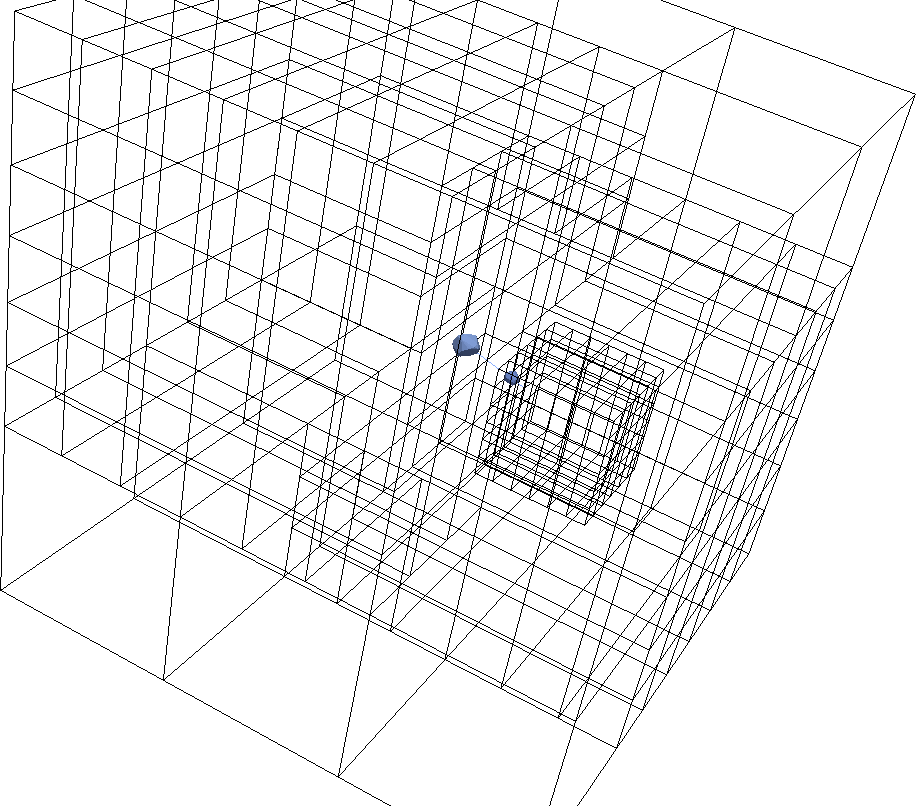
\includegraphics[width=0.3\textwidth]{experiments/two-bodies/visualisation/adaptive-grid01.png}
    \hspace{0.2cm}
    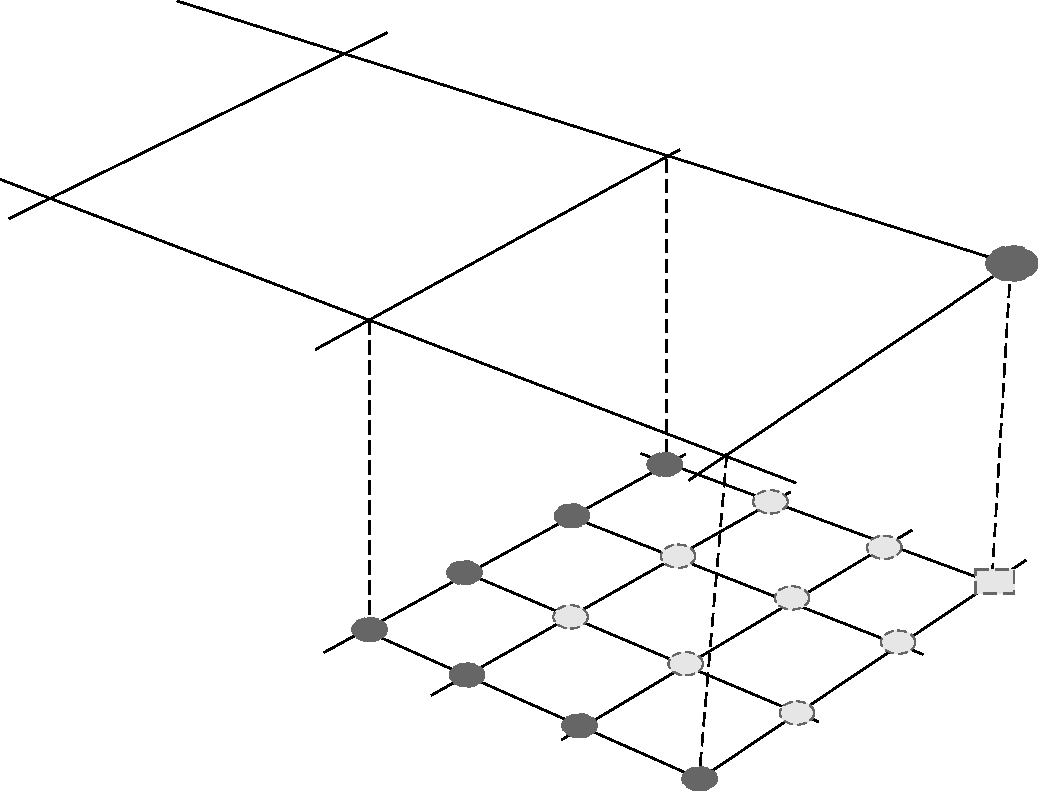
\includegraphics[width=0.3\textwidth]{sketches/multigrid.pdf}
  \end{center}
  \caption{
    Left: Whenever the grid traversal enters a cell, it checks whether particles
    assigned to one vertex do collide with particles assigned to another vertex.
    To avoid redundant collision computations, we check only some vertex pairs
    (dotted, larger lines).
    Middle: Two particles approach each other. As they are of different size,
    they might be held on different spacetree resolution levels.
    Right: In the adaptive case, particles are dropped from the coarse levels
    into the fine grid (rectangular marker) if new grid levels are added. The
    bright round vertices are children of the marked coarse grid vertex. The
    bright and the dark round markers' vertices together are the descendants of
    the marked coarse grid vertex.
  }
  \label{figure:collision-cube}
\end{figure}


We then write down the algorithm as a set of events, i.e.~we specify which
operations are performed if a vertex is read for the very first time \linebreak
(\texttt{touchVertexFirstTime}), if a cell is entered
(\texttt{enterCell}), and so forth.
Besides the actual grid hosting the particles, the grid sweeps build and
maintain two further sets of collision points (algorithm \ref{algorithm:grid-based-dem}).

\begin{algorithm}
 \caption{A grid-based DEM implementation.}
 \label{algorithm:grid-based-dem}
 \begin{algorithmic}[1]
  \Function{traverseGrid}{$\mathcal{C}$}
   \State $\mathcal{C}_{old} \gets \mathcal{C}$
   \State $\mathcal{C} \gets \emptyset$
   \While{traversal continues}
    \If{\texttt{touchVertexFirstTime}}
     \ForAll{particles $p$ associated to vertex}
      \ForAll{contact points $c \in \mathcal{C}_{old}$ associated to $p$}
       \State Update $f(p)$ through $c$
      \EndFor
      \State Update particle incl.~its triangles
     \EndFor
     \ForAll{particle pairs $(p_i,p_j)$ associated to vertex}
       \State $\mathcal{C} \gets \mathcal{C} \cup $
       \Call{findCollisions}{$p_i,p_j$}
     \EndFor
    \EndIf
    \If{\texttt{enterCell}}
     \ForAll{$2^d$ vertices adjacent to cell}
      \ForAll{particles $p$ associated to vertex}
       \If{particle should be associated to different vertex}
        \State Reassign particle
       \EndIf
      \EndFor
     \EndFor
     \ForAll{$(p_i,p_j)$ associated to different vertices (cmp.~figure)} 
      \State $\mathcal{C} \gets \mathcal{C} \cup $
       \Call{findCollisions}{$p_i,p_j$}
     \EndFor
    \EndIf
   \EndWhile
  \EndFunction

  %\Function{main}{$T$}   
  % \State $\mathcal{C} \gets \emptyset $
  % \State $t \gets 0 $
  % \For{$t < T$}
  %  \State \Call{traverseGrid}{$\mathcal{C}$}
  %  \State $t \gets t + \Delta t$
  % \EndFor
  %\EndFunction
 \end{algorithmic}
\end{algorithm} 


Our grid-based realisation is characterised by few properties:
\begin{itemize}
  \item When we load a vertex for the very first time, we make all particles
  associated to this vertex move. 
  \item When we load a vertex, we do compare all the particles associated to
  this vertex with each other and identify collision points. The comparison of
  particles associated to different vertices is realised when we enter a cell.
  Here, we do compare the vertex pairs from Figure \ref{figure:collision-cube}---left bottom
  front vertex with right bottom front vertex, all diagonal combinations, and
  so forth---such that we avoid multiple evaluations of vertex pairs. For 
  boundary cells, some special case distinctions yielding additional checks are
  added. If a cell is traversed, we assume that all its adjacent vertices are
  available, i.e.~have been read before.
  \item Whenever we run into a cell, we run through all the adjacent vertices
  and their particles. They all already have an updated position, as any vertex
  has been loaded before and thus been subject to \texttt{touchVertexFirstTime}.
  If a particle is associated to the 'wrong' vertex as it has moved and should 
  be assigned to another vertex of the cell, we do the reassignment. A particle
  may move at most one cell of its corresponding level a time.
  \item The vertex comparisons yield a set of collision points. This set is kept
  persistent for the subsequent traversal: one time step of the scheme is
  realised per two grid traversal. The amortised cost however still is one time
  step per grid traversal. This scheme picks up the idea of pipelining
  \cite{Plimpton1995}. Collision data is mapped onto the particles when we read a
  particle for the first time in the subsequent traversal. Immediately after the
  forces acting on a particle are determined, we do update the particle's
  property and also update the geometric data due to translation and rotation.
\end{itemize}

\noindent
The extension of the present scheme to multiscale trees is detailed below.
To make the algorithm correct, each contact point set between two particles does
exist twice with inverse normals.
Each set furthermore is augmented with a copy of the corresponing partner
particles' global data (mass, velocity, momentum).
Otherwise, we would have to search for this data and build up global indices,
and have to be aware that the particle's data already might have been subject to
the next time step.


\begin{observation}
The algorithm realises a single-pass policy. Geometric data is written only once
per traversal, and is read only when we read in a vertex for the first time and
when we run through a cell.
The implementation's pressure on the memory subsystem thus is minimalistic as
long as the spatial and temporal grid access locality \cite{dime} is high which
yields high cache hit rates.
We rely on a space-filling curve to
run through the grid \cite{Weinzierl:2009:Diss,Weinzierl:11:Peano} and thus
guarantee such a two-fold locality.
\end{observation}


\noindent
More sophisticated explicit schemes can be realised with the same single-touch
policy if we hold additional data per particle (acceleration, e.g.).
Such an approach picks up ideas of pipelining \cite{Plimpton1995}.




{\bf Regular grid.}
The spacetree formalism allows us to realise at least three grid variants. 
A very simple refines all spacetree nodes all the time as long as the resulting
cell mesh size is bigger than the largest particle diameter.
Such a strategy yields a regular Cartesian grid. 

{\bf Dynamically adaptive grid.}
Our dynamically adaptive grid is characterised by two ingredients: mesh
refinement control and inter-grid particle treatment.
In \texttt{touchVertexFirstTime}, our code analyses what the smallest diameter
of all the particles held by the vertex is.
If this diameter is smaller than $1/3$ of the mesh width corresponding to the
vertex's level, then the region around the vertex is refined.
If we run into a vertex, we check whether there are any spatially coinciding
vertices in the tree on a coarser level.
If such vertices do exist, we run through all of their particles and move them
one level down if the diameter permits.
The scheme successively drops the particles down the grid hierarchies.

\begin{figure}
 \begin{center}
  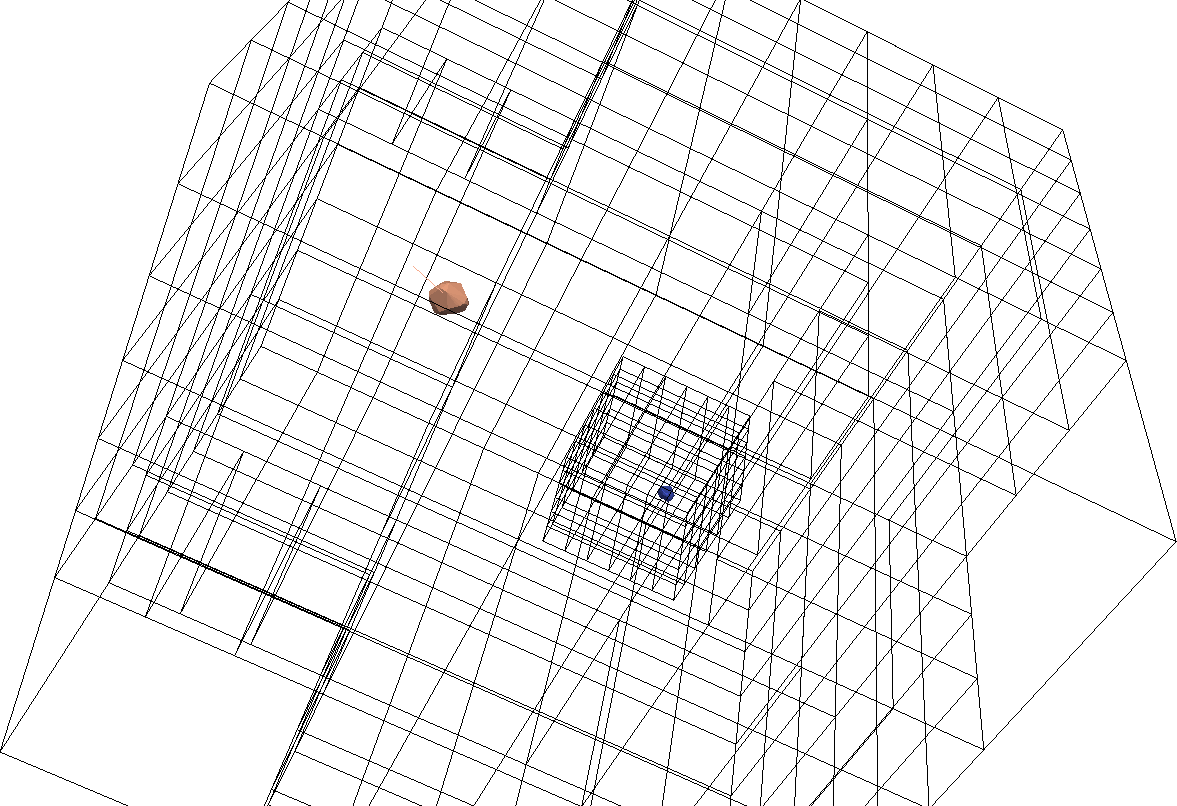
\includegraphics[width=0.4\textwidth]{experiments/two-bodies/visualisation/adaptive-grid00.png}
  \hspace{1.1cm}
  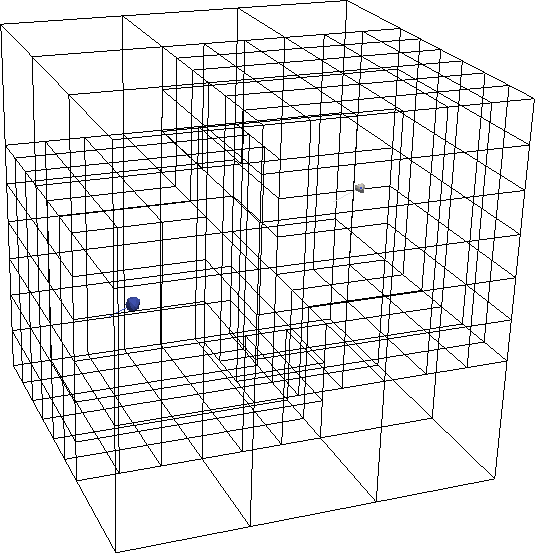
\includegraphics[width=0.25\textwidth]{experiments/two-bodies/visualisation/reluctant-adaptive-grid00.png}
  \\
  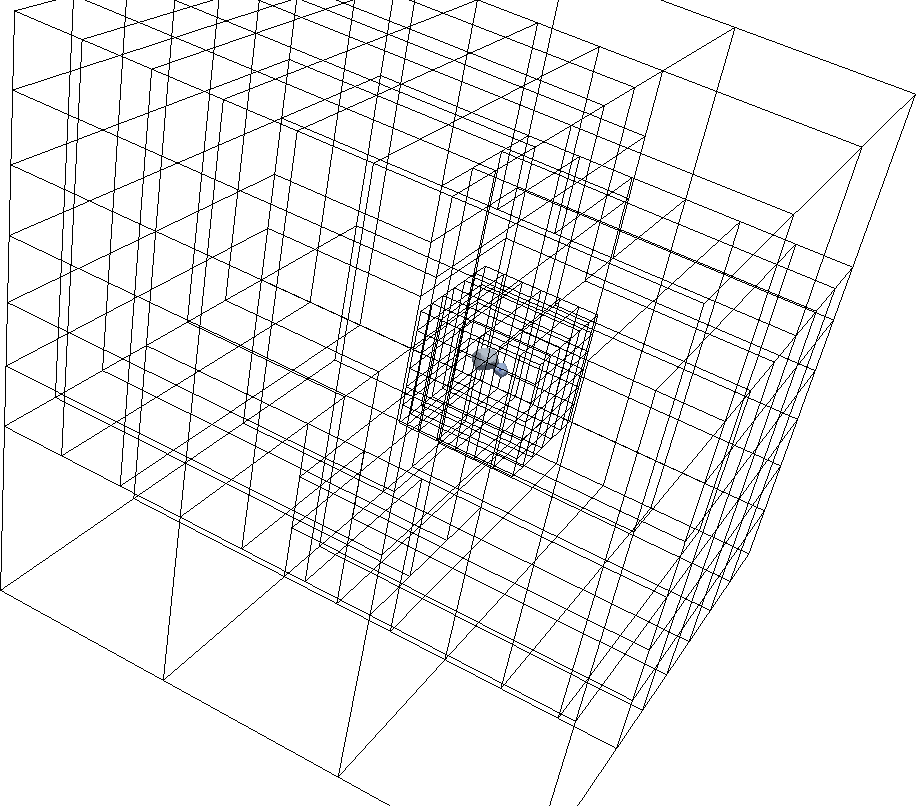
\includegraphics[width=0.3\textwidth]{experiments/two-bodies/visualisation/adaptive-grid02.png}
  \hspace{1.1cm}
  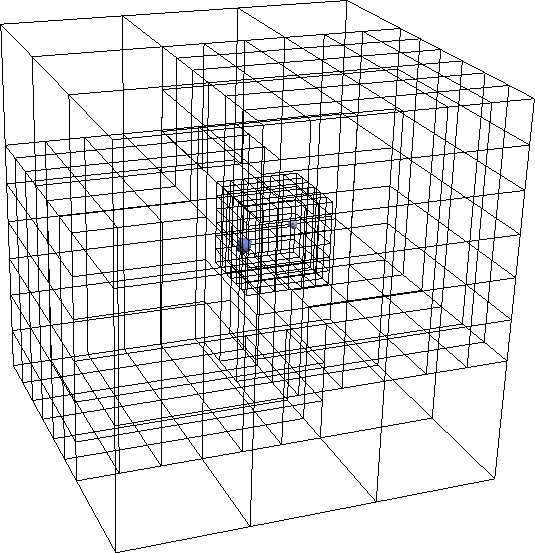
\includegraphics[width=0.3\textwidth]{experiments/two-bodies/visualisation/reluctant-adaptive-grid02.png}
% 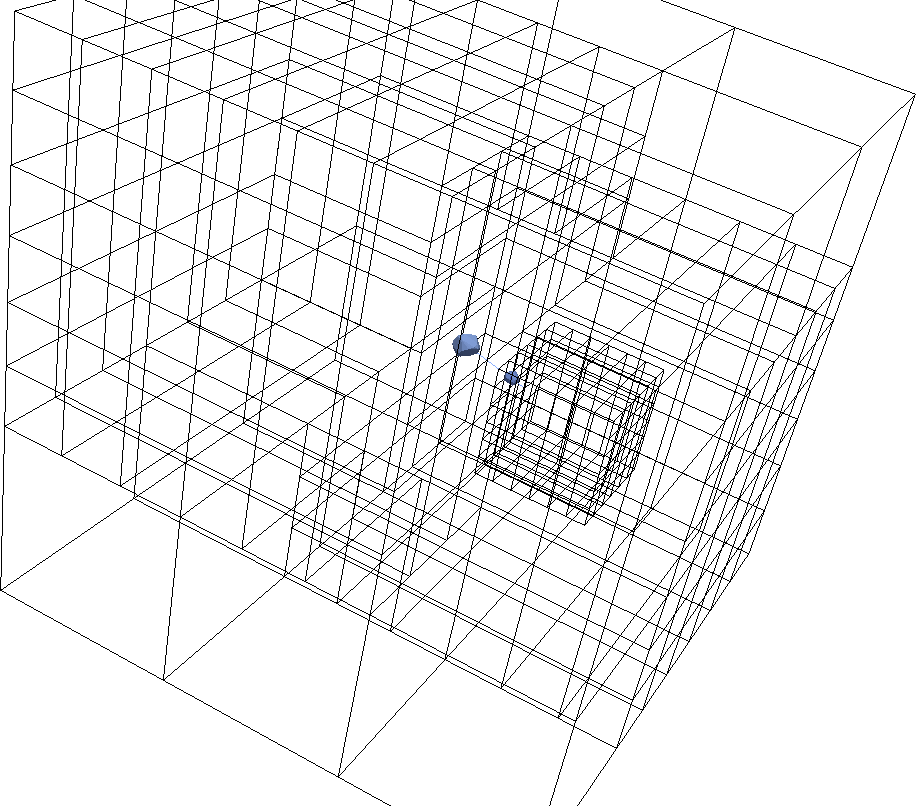
\includegraphics[width=0.3\textwidth]{experiments/two-bodies/visualisation/adaptive-grid01.png}
%   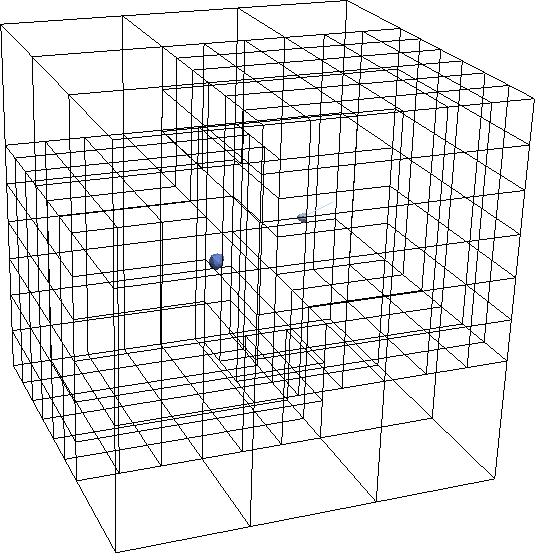
\includegraphics[width=0.3\textwidth]{experiments/two-bodies/visualisation/reluctant-adaptive-grid01.png}\\
%   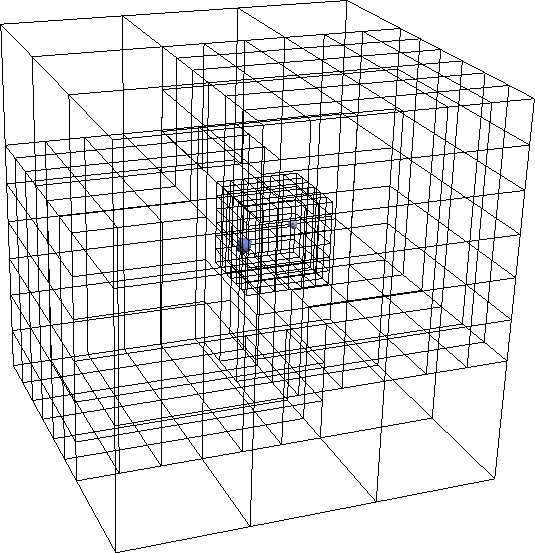
\includegraphics[width=0.3\textwidth]{experiments/two-bodies/visualisation/reluctant-adaptive-grid02.png}
%   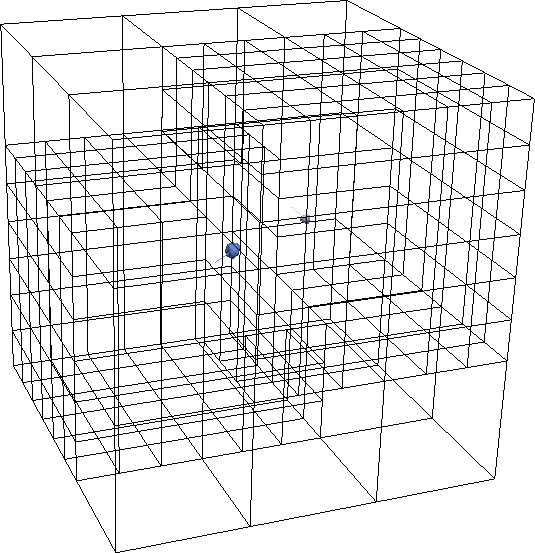
\includegraphics[width=0.3\textwidth]{experiments/two-bodies/visualisation/reluctant-adaptive-grid03.png}\\
 \end{center}
 \caption{
   Two particles crash into each other.
   The adaptive grid refining around each particle while its diameter
   constrains the mesh size (left column).
   The reluctant adaptive grid works with a coarser resolution as long
   as particles are far away from each other (right column).
   Just before they collide, the grid is refined and particles are dropped down
   the resolution levels.
 }
 \label{figure:adaptive-vs-reluctant-grid}
\end{figure}


We define two multiscale relationships between vertices (Figure
\ref{figure:collision-cube}).
A vertex $a$ is a child of a vertex $b$ if all adjacent cells of $a$ are
children of adjacent cells of $b$.
$b$ is the parent vertex of $a$.
A vertex $a$ is a descendant of $b$ if at least one adjacent cell of $a$ is a
child of an adjacent cell of $b$.
$b$ is an ancestor of $a$.
If we delete a vertex $a$ that holds particles, its particles are moved to the
next coarser level and assigned there to the nearest parent of $a$.
Each vertex holds a boolean marker that is set $\bot $ before the vertex is
read for the first time.
If a vertex holds a particle, all the markers of the vertices where it is a
descendent from are set to $\top$.
If a vertex whose adjacent cells all are refined holds $\bot$ at the end of the
multiscale traversal, we coarsen these refined adjacent cells.
We rely on a top-down tree traversal.
The refinement/coarsening procedure then can be evaluated on-the-fly.
It equals an analysed tree grammar \cite{knuth}.

For the multiscale contact detection, we extend the list of particles associated
to a vertex. 
There is the list of actually held particles and a list of virtual particles. 
We run through the grid top down, i.e.~a vertex always is read for the first
time before any of its descendants, and clear virtual particle list first.
Then, we add all particles held in the particle or the virtual particle lists of
any ancestor to the local virtual list.
If we compare all particles with each other that are held by the same vertex, we
do compare the actual particles with all other real particles as well as all
virtual particles.


{\bf A reluctant adaptive grid.}
The dynamically adaptive grid refines rather aggressive: Particles are always
dropped to their corresponing refinement level immediately. 
Fine grid regions thus follow `their' particles (Figure
\ref{figure:adaptive-vs-reluctant-grid}).
This might introduce finer grids than actually required for contact detection
which is an overhead.
Given the one-cell-per-time-step constraint on the particle velocity, we also
restrict the maximum velocity or time step rigorously.
For the present work, this does not have a major impact as we apply uniform
small time step sizes globally. 
For schemes with local time stepping, it however is important, besides overhead
discussions, to keep the grid as coarse as possible as this facilitates big
time step sizes.


Our reluctant adaptive grid works with coarser adaptive grids than the plain
variant through two modifications of the refinement procedure: 
On the one hand, we refine the region around a vertex if the previous criterion
holds and the vertex holds at least two particles.
If only one particle is holds, we stick locally to the grid no matter what the
particular diameter is.
Throughout the inter-vertex contact detection in \texttt{enterCell}, we further
bookkeep the minimum diameter of all the particles involved. 
If this minimal diameter is smaller than the cell, we do refine this cell, too.


